\chapter{La integral de convolución}

\section{Deducci\'{o}n de la f\'{o}rmula}

A continuaci\'{o}n calculamos la salida $y(t)$ para una entrada arbitraria $x(t)$ en función de la respuesta al impulso $h(t)$ del sistema lineal invariante en el tiempo.

\subsection{Una se\~{n}al como l\'{\i}mite de una sumatoria}

\begin{figure}
	\centering
	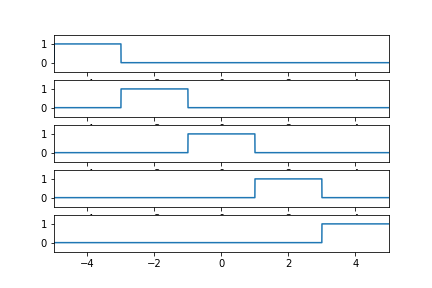
\includegraphics[width=0.7\linewidth]{graphics/pulses}
	\caption{Pulsos desplazados en el tiempo}
	\label{fig:pulses}
\end{figure}

\begin{figure}
	\centering
	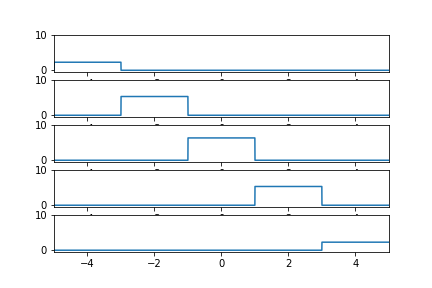
\includegraphics[width=0.7\linewidth]{graphics/modulated_pulses}
	\caption{Pulsos desplazados en el tiempo y modulados}
	\label{fig:modulatedpulses}
\end{figure}

\begin{figure}
	\centering
	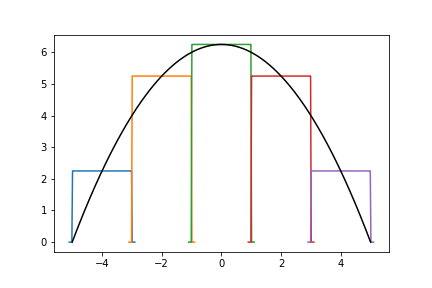
\includegraphics[width=0.7\linewidth]{graphics/coarse-approximation}
	\caption{Aproximación grosera}
	\label{fig:coarse-approximation}
\end{figure}

\begin{figure}
	\centering
	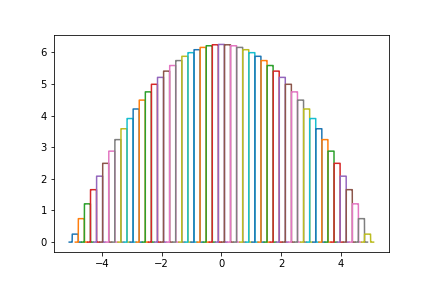
\includegraphics[width=0.7\linewidth]{graphics/fine-approximation}
	\caption{Aproximación fina}
	\label{fig:fine-approximation}
\end{figure}

Vamos a probar que podemos representar una se\~{n}al 
continua como el l\'{\i}mite de una suma de pulsos.
Consideremos pulsos desplazados en el tiempo $\delta _{\Delta }\left(t-k \, \Delta \right)$ 
donde $\Delta$ es un incremento de tiempo variable. 
Observando la figura \ref{fig:pulses}, podemos escribir las definiciones de los pulsos desplazados en el tiempo
\begin{equation}
        \begin{array}{c}
                ...                                             \\ 
                \delta _{\Delta }\left( t+\Delta \right) =
                        \left\{ \begin{array}{l}
                                        \frac{1}{\Delta },      \\ 
                                        0,
                                \end{array}
                                \begin{array}{l}
                                        -\Delta \leq t<0,       \\ 
                                        \left( t<-\Delta \right) \vee \left( 0\leq t\right) ,
                                \end{array}
                        \right.                                 \\ 
                \delta _{\Delta }\left( t\right) =
                        \left\{ \begin{array}{l}
                                        \frac{1}{\Delta },      \\ 
                                        0,
                                \end{array}
                                \begin{array}{l}
                                        0\leq t<\Delta ,        \\ 
                                        \left( t<0\right) \vee \left( \Delta \leq t\right) ,
                                \end{array}
                        \right.                                 \\ 
                \delta _{\Delta }\left( t-\Delta \right) =
                        \left\{ \begin{array}{l}
                                        \frac{1}{\Delta },      \\ 
                                        0,
                                \end{array}
                                \begin{array}{l}
                                        \Delta \leq t<2 \, \Delta , \\ 
                                        \left( t<\Delta \right) \vee \left( 2 \, \Delta \leq t\right) ,
                                \end{array}
                        \right.                                 \\ 
                ...                                             \\ 
                \delta _{\Delta }\left( t-k \, \Delta \right) =
                        \left\{ \begin{array}{l}
                                        \frac{1}{\Delta },      \\ 
                                        0,
                                \end{array}
                         \begin{array}{l}
                            k \, \Delta \leq t<\left( k+1\right) \, \Delta , \\ 
                              \left( t<k \, \Delta \right) \vee \left( \left( k+1\right) \, \Delta \leq t\right) .
                         \end{array}
               \right.
        \end{array}
\end{equation}
Multiplicando por $x\left( k \, \Delta \right) \, \Delta $ al $k-\acute{e}simo$ pulso (ver figura \ref{fig:modulatedpulses}) se obtiene 
\begin{equation}
        \begin{array}{c}
                        ...                                                                    \\ 
                        x\left( -\Delta \right) \, \delta _{\Delta }\left( t+\Delta \right) \, \Delta =
                                \left\{ \begin{array}{l}
                                                \frac{x\left( -\Delta \right) }{\Delta } \, \Delta ,        \\ 
                                                0,
                                        \end{array}
                                        \begin{array}{l}
                                           -\Delta \leq t<0,                                       \\ 
                                          \left( t<-\Delta \right) \vee \left( 0\leq t\right) ,
                                        \end{array}
                                \right.                                                                 \\ 
                        x\left( 0\right) \, \delta _{\Delta }\left( t\right) \, \Delta =
                                \left\{ \begin{array}{l}
                                                \frac{x\left( 0\right) }{\Delta } \, \Delta ,               \\ 
                                                0,
                                        \end{array}
                                        \begin{array}{l}
                                                0\leq t<\Delta ,                                        \\ 
                                                \left( t<0\right) \vee \left( \Delta \leq t\right) ,
                                        \end{array}
                                \right.                                                                 \\ 
                        x\left( \Delta \right) \, \delta _{\Delta }\left( t-\Delta \right) \, \Delta =
                                \left\{ \begin{array}{l}
                                                \frac{x\left( \Delta \right) }{\Delta } \, \Delta ,         \\ 
                                                0,
                                        \end{array}
                                        \begin{array}{l}
                                                \Delta \leq t<2 \, \Delta ,                                 \\ 
                                                \left( t<\Delta \right) \vee \left( 2 \, \Delta \leq t\right) ,
                                        \end{array}
                                \right.                                                                 \\ 
                        ... \\ 
                        x\left( k\Delta \right) \, \delta _{\Delta }\left( t-k\Delta \right) \, \Delta =
                                \left\{ \begin{array}{l}
                                                \frac{x\left( k \, \Delta \right) }{\Delta } \, \Delta ,        \\ 
                                                0,
                                        \end{array}
                       \begin{array}{l}
                             k \, \Delta \leq t<\left( k+1\right) \, \Delta ,               \\ 
                             \left( t<k \, \Delta \right) \vee \left( \left( k+1\right) \, \Delta \leq t\right) .
                       \end{array}
                       \right.
        \end{array}
\end{equation}
Observe que un valor dado de $t$ (por ejemplo $t_{0})$ s\'{o}lo puede pertenecer a \textbf{un} intervalo 
$k\Delta \leq t<\left( k+1\right) \Delta,$ por lo tanto para $t_{0}$ solo uno de los productos puede ser 
distinto de $0$. Sumando los infinitos productos (ver figura \ref{fig:coarse-approximation}) obtenemos 
\begin{equation}
   x_{\Delta }\left( t\right) =
     \sum_{k=-\infty }^{\infty }x\left( k\Delta \right) \, \delta _{\Delta }\left( t-k \, \Delta \right) \, \Delta .
\end{equation}

%\begin{figure*}[ht]
%\begin{center}
%\includegraphics[scale=.70]{./graphics/contcont222.eps}
%\end{center}
%\caption{Se\~{n}ales como suma de pulsos}
%\label{contcont222eps}
%\end{figure*}

Considerando la suma de los pulsos desplazados en el tiempo 
podemos observar que cuando $\Delta $ tiende a cero (ver figura \ref{fig:fine-approximation}) $x_{\Delta }\left( t\right) $ tiende a $x\left( t\right).$
\begin{equation}
        x\left( t\right) =      
\begin{array}{l}
    Lim \\ 
    \Delta \rightarrow 0
\end{array}
x_{\Delta }\left( t\right) = 
\begin{array}{l}
    Lim \\ 
    \Delta \rightarrow 0
\end{array}
   \sum_{k=-\infty }^{\infty }x\left( k \, \Delta \right) \, \delta _{\Delta }\left(t-k \, \Delta \right) \, \Delta .
\end{equation}
Adem\'{a}s, cuando $\Delta $ tiende a cero, la sumatoria se convierte en una integral 
\begin{equation}
        x\left( t\right) =\int_{-\infty }^{\infty }x\left( \tau \right) \, \delta\left( t-\tau \right) \, d\tau .
        \label{integral.convolucion}
\end{equation}

Notemos que por la propiedad del muestreo, debe cumplirse 
\begin{equation} 
     x\left( t\right) \, \delta \left( t-\tau \right) =
   x\left( \tau \right) \, \delta \left( t-\tau \right),
\end{equation}
y en ese caso 
\begin{equation}
 x\left( t\right) = 
  x\left( t\right) \, \left( \int_{-\infty }^{\infty } \delta \left( t-\tau \right) \, d\tau \right) .
\end{equation}

\subsection{La respuesta al impulso y la convolución}

Definamos $h_{k \, \Delta }(t) = h_{\Delta }\left( t-k \, \Delta \right)$ como la salida de un sistema invariante en el tiempo para el pulso 
$\delta _{\Delta }(t-k \, \Delta ).$ 

Además, recordemos la ecuaci\'{o}n (\ref{integral.convolucion})
\begin{equation}
 x_{\Delta }\left( t\right) =
  \sum_{k=-\infty }^{\infty }x\left( k \, \Delta \right) \, \delta _{\Delta }\left( t-k \, \Delta \right) \, \Delta ,
\end{equation}

La salida $y_{\Delta }\left( t\right) $ para una entrada $x_{\Delta }\left( t\right) $ puede 
definirse, por el principio de superposici\'{o}n, como 
\begin{equation}
        y_{\Delta }\left( t\right) =
        \sum_{k=-\infty }^{\infty }x\left( k\Delta \right) \, h_{k\Delta }\left( t\right) \, \Delta
\end{equation}
 
Definamos $k\Delta =\tau .$ Entonces, cuando $\Delta \rightarrow 0,$ obtenemos como l\'{\i}mite la 
se\~{n}al $y(t),$ pero como siempre vamos a tener un $k$ suficientemente grande $\tau $ no es 
necesariamente nula. Podemos escribir 
\begin{equation}
        y\left( t\right) = 
                \begin{array}{l}
                        Lim \\ 
                        \Delta \rightarrow 0
                \end{array}
                \sum_{k=-\infty }^{\infty }x\left( k \, \Delta \right) \, h_{k\Delta }\left(t\right) \, \Delta =
                        \int_{-\infty }^{\infty }x\left( \tau \right) \, h_{\tau}\left( t\right) \, d\tau ,
\end{equation}

Si el sistema es invariante en el tiempo, entonces 
\begin{equation}
h_{\tau }\left( t\right) =h_{0}\left( t-\tau \right) ,
\end{equation}
(es decir, no importa para que $\tau $ calculamos la respuesta, y por lo tanto elegimos $\tau =0$), y por 
lo tanto obtenemos la integral de convolución 
\begin{equation}
        y\left( t\right) =\int_{-\infty }^{\infty }x\left( \tau \right) \, h\left(t-\tau \right) \, d\tau .
\end{equation}

%\section{La integral de convolución paso a paso}
%
%Para calcular la convolución 
%\begin{equation}
%     y\left( t\right) =\int_{-\infty }^{\infty }x\left( \tau \right) \, h\left(t-\tau \right) \, d\tau .
%\end{equation}
%en el momento $t = t_{0}$, debemos ejecutar los siguientes pasos
%\begin{enumerate}
%\item Dada $h(\tau)$, reemplazar la variable independiente $\tau$ por $-\tau$ para obtener
%  $h(-\tau)$, la  versi\'{o}n reflejada respecto a $\tau = 0$.
%\item desplazar $h(-\tau)$ a la posici\'{o}n $t_{0}$, o en
%  otras palabras, se desplaza $h(-\tau)$ de forma tal que el valor
%  original $h(0)$ esté ubicado en $\tau = \tau_{0}$.
%\item evaluar el producto $z(t_{0},\tau) = x(\tau) \, h(t_{0} - \tau)$.
%\item evaluar la integral $y(t_{0}) = \int_{v=-\infty}^{\infty} z(t_{0},\tau) \, d\tau$.
%\end{enumerate}

\section{Cálculo de la suma de convolución en forma gr\'{a}fica}


El c\'{a}lculo de la convolución tiene una interpretaci\'{o}n
gr\'{a}fica.
\begin{enumerate}
\item Consideremos la f\'{o}rmula
  \begin{equation}
    y\left(t\right) = \int_{-\infty }^{\infty }x\left(v\right) \, h\left(t - v\right) \, dv.
    \label{concontgraf}
  \end{equation}
        
\item En la ec. (\ref{concontgraf}) el factor $h(t - v)$ es una
  versi\'{o}n de $h(v)$ invertida en el tiempo (observe la variable
  $v$ en ambas funciones) y desplazada en el tiempo con desplazamiento $t$, la variable independiente $t$ de la salida $y(t)$.
       
        
\item En base a la observación anterior, es posible enunciar la
  siguiente ``receta'' para calcular la convolución en forma
  gr\'{a}fica.
  \begin{enumerate}
  \item Dibuje la se\~{n}al $x(v)$.
                
  \item Invierta en el tiempo la se\~{n}al $h(v)$ para obtener $h(-v)$.
                
  \item Repita los siguientes pasos para calcular distintos valores de
    $y(t)$
    \begin{enumerate}
                
    \item Desplace en el tiempo la se\~{n}al $h(-v)$ para obtener $h(t-v)$.
                        
    \item Obtenga el producto $z(v,t) = x(v) \, h(t - v)$.
                        
    \item El valor de $y(t)$ es $\int z(v,t) \, dv$
                        
    \end{enumerate}
  \end{enumerate}
\end{enumerate}

\section{Ejemplos}


\subsection{Convolución de una señal con un impulso desplazado}

Supongamos la entrada $x(t) = \delta(t- a)$ a un sistema linear invariante en el tiempo con respuesta al impulso $h(t)$.
En este caso la salida es
\begin{equation}
 y(t) = \int_{-\infty}^{\infty} \delta(v - a) \, h(t - v)  \, dv
\end{equation}
Notemos el producto $\delta(v - a) \, h(t - v) = h(t - a) \, \delta(v - a)$,
donde $v = a$. Por lo tanto
\begin{equation}
 y(t) = \int_{-\infty}^{\infty} h(t - a) \, \delta(v - a ) \, dv,
\end{equation}
\begin{equation}
 y(t) = h(t - a) \, \left( \int_{-\infty}^{\infty} \delta(v - a ) \, dv\right).
\end{equation}
Recordemos que por definición de impulso
\begin{equation}
 \int_{-\infty}^{\infty} \delta(v - a ) \, dv = 1.
\end{equation}
Por lo tanto
\begin{equation}
 y(t) = h(t - a),
\end{equation}
y así comprobamos la invariancia en el tiempo de los sistemas cuya salida $y(t)$ para una entrada $x(t)$ puede calcularse con la integral de convolución.


\subsection  {Dos se\~{n}ales infinitas}

\begin{enumerate}

\item Sean dos se\~{n}ales definidas como
\begin{eqnarray}
        x\left( t\right) &=& e^{2 \, t} \, u\left( -t\right) ,  \\
        h\left( t\right) &=& u\left( t-3\right).
\end{eqnarray}

\item Calculando la suma de convolución tenemos
\begin{equation}
        x\left( t\right) * h\left( t\right) = 
        \int_{-\infty }^{\infty}e^{2 \, \tau} u\left( - \tau\right) u\left( t-3-\tau \right) d\tau ,
\end{equation}

\item El producto $u\left( -\tau\right) u\left( t-3-\tau \right)$ puede analizarse así:
\begin{enumerate}
\item Debemos observar las transiciones de los escalones: donden cambian de $0$ a $1$ y viceversa. Estas
transiciones determinan los límites de las integrales, porque si el integrando es nulo (o sea, si 
alguno de los escalones incluidos como factores en el integrando tiene un argumento negativo) entonces
la integral se anula también en un intervalo de tiempo determinado.
\item Para este caso
\item Para $t < 3$,
\begin{equation}
        t < 3   \rightarrow  u\left( -\tau\right) u\left( t-3-\tau \right) = 
        u\left( t-3-\tau \right),
\end{equation}
\begin{equation}
        t<3 \rightarrow x\left( t\right) * h\left( t\right) = \int_{-\infty}^{t-3}e^{2\tau}d\tau ,
\end{equation}

\item Para $t \geq 3$,
\begin{equation}
        t \geq 3        \rightarrow  u\left( -\tau\right) u\left( t-3-\tau \right) = 
        u\left( -\tau \right),
\end{equation}
y
\begin{equation}
        t\geq 3 \rightarrow x\left( t\right) * h\left( t\right) = \int_{-\infty}^{0}e^{2\tau}d\tau .
\end{equation}
\end{enumerate}
\end{enumerate}

\subsection{Un par de señales limitadas en tiempo}

\begin{enumerate}

\item Sean las se\~{n}ales
\begin{equation}
  x\left( t\right) =u\left( t\right) -u\left( t-4\right),
\end{equation}
y
\begin{equation}
h\left( t\right) =\cos \left( \frac{\pi t}{2}\right) \left( u\left( t\right)-u\left( t-4\right) \right),
\end{equation}

\item Planteando la integral de convolución, obtenemos
\begin{equation}
        x\left( t\right)  * h\left( t\right) =
                \int_{-\infty }^{\infty }
                        \cos \left( \frac{\pi \tau}{2}\right) 
                        \left( u\left( \tau \right) - u\left( \tau -4\right) \right)
                        \left( u\left( t-\tau \right) - u\left( t-4-\tau \right) \right) d\tau ,
\end{equation}

\item Finalmente, obtenemos
\begin{equation}
        t<0, \, x\left( t\right) * h\left( t\right) =0,
\end{equation}
\begin{equation}
        4>t\geq 0, \, x\left( t\right) * h\left( t\right) =
                \int_{0}^{t}\cos\left( \frac{\pi \tau}{2}\right) d\tau ,
\end{equation}
\begin{equation}
        8>t\geq 4, \, x\left( t \right)  h\left( \right) =
                \int_{t-4}^{4}\cos\left( \frac{\pi t}{2}\right) d\tau ,
\end{equation}
y
\begin{equation}
        t\geq 8, \, x\left( t\right)  h\left( t\right) =0.
\end{equation}

\end{enumerate}

\subsection{Otro par de señales limitadas en tiempo}

\begin{enumerate}

\item Sean dos se\~{n}ales definidas por
\begin{eqnarray}
        x\left( t\right) &=&
                \left\{ \begin{array}{cc}
                                1 & 0<t<T,                                                       \\ 
                                0 & \left( t\leq 0\right) \vee \left( T\leq t\right) ,
                        \end{array}
                \right.                                                                       \\
        h\left( t\right) &=&
                \left\{ \begin{array}{cc}
                                t & 0<t<T,                                                       \\ 
                                0 & \left( t\leq 0\right) \vee \left( T\leq t\right).
                        \end{array}
                \right.
\end{eqnarray}
En otras palabras (o mejor dicho, f\'{o}rmulas)
\begin{equation}
        x\left( t\right) = u\left( t\right) -u\left( t-T\right) ,
\end{equation}
y
\begin{equation}
        h\left( t\right) = t \, \left( u\left( t\right) -u\left( t-T\right) \right).
\end{equation}

\item Invirtiendo y desplazando en el tiempo una de las se\~{n}ales, tenemos
\begin{equation}
        h\left( t-\tau \right) = 
        \left( t-\tau \right) \, \left( u\left( t-\tau \right)-u\left( t-\tau -T\right) \right) .
\end{equation}

\item Finalmente, calculamos la integral
\begin{equation}
        f\left( t\right) =
        \int_{-\infty}^{\infty}    
                \left( u\left( \tau\right) -u\left(\tau-T\right) \right) \,
                \left( t-\tau \right) \, \left( u\left( t-\tau \right) -u\left( t-\tau-T\right) \right) 
        \, d\tau
\end{equation}
\begin{equation}
        f\left( t\right) =
        \int_{-\infty}^{\infty}
                \left( t-\tau \right) \, \left( u\left( t\right)-u\left( t-T\right) \right) \, 
                \left( u\left( t-\tau \right) -u\left( t-T-\tau \right) \right) \, d\tau
\end{equation}
\begin{eqnarray}
        t &<&0  \rightarrow f\left( t\right) =0,                                                     \\
        0 &\leq &t<T\rightarrow f\left( t\right) =
        \left[ t \, \tau -\frac{\tau ^{2}}{2}\right] _{0}^{t}=\frac{t^{2}}{2},            \\
        T &\leq &t<2 \, T\rightarrow f\left( t\right) =
        \left[ t \, \tau -\frac{\tau ^{2}}{2}\right] _{t-T}^{T}=-\frac{t^{2}}{2}+t \, T.     \\
        2 \, T &\leq &t\rightarrow f\left( t\right) =0.
\end{eqnarray}

\end{enumerate}
